\section{Evaluation} \label{sec:eval}

In this section, we evaluate the scalability of designs generated by \name.
We also compare the absolute performance of a Plasticine chip compiled with \name against a Tesla V100 GPU 
for a mix of deep learning, sorting, graph processing, and streaming applications.

For our baseline implementation on GPU, we use frameworks and libraries whenever possible, such as TensorFlow compiled
with cuDNN library for deep learning and Gunrock library~\cite{gunrock} for graph applications.
When no library is available, we implement and hand optimize the CUDA implementation.

To better match the V100's peak FLOPS, 
we increase the Plasticine array from a $16\times8$ to a $20\times20$ configuration.
The area footprint of this configuration is \SI{352}{mm^2} at 28nm, which is still well below the 
\SI{815}{mm^2} at 12nm for V100.
We could not match in die area, as the speed of our cycle-accurate simulator limits our selection of Plasticine size.
To match in GPU's off-chip bandwidth, 
we integrate an open-source DRAM simulator--Ramulator~\cite{ramulator}--with our
cycle-accurate simulator to model the HBM2 technology, providing a \SI{1}{TB/s} off-chip bandwidth.

\begin{figure*}
\centering
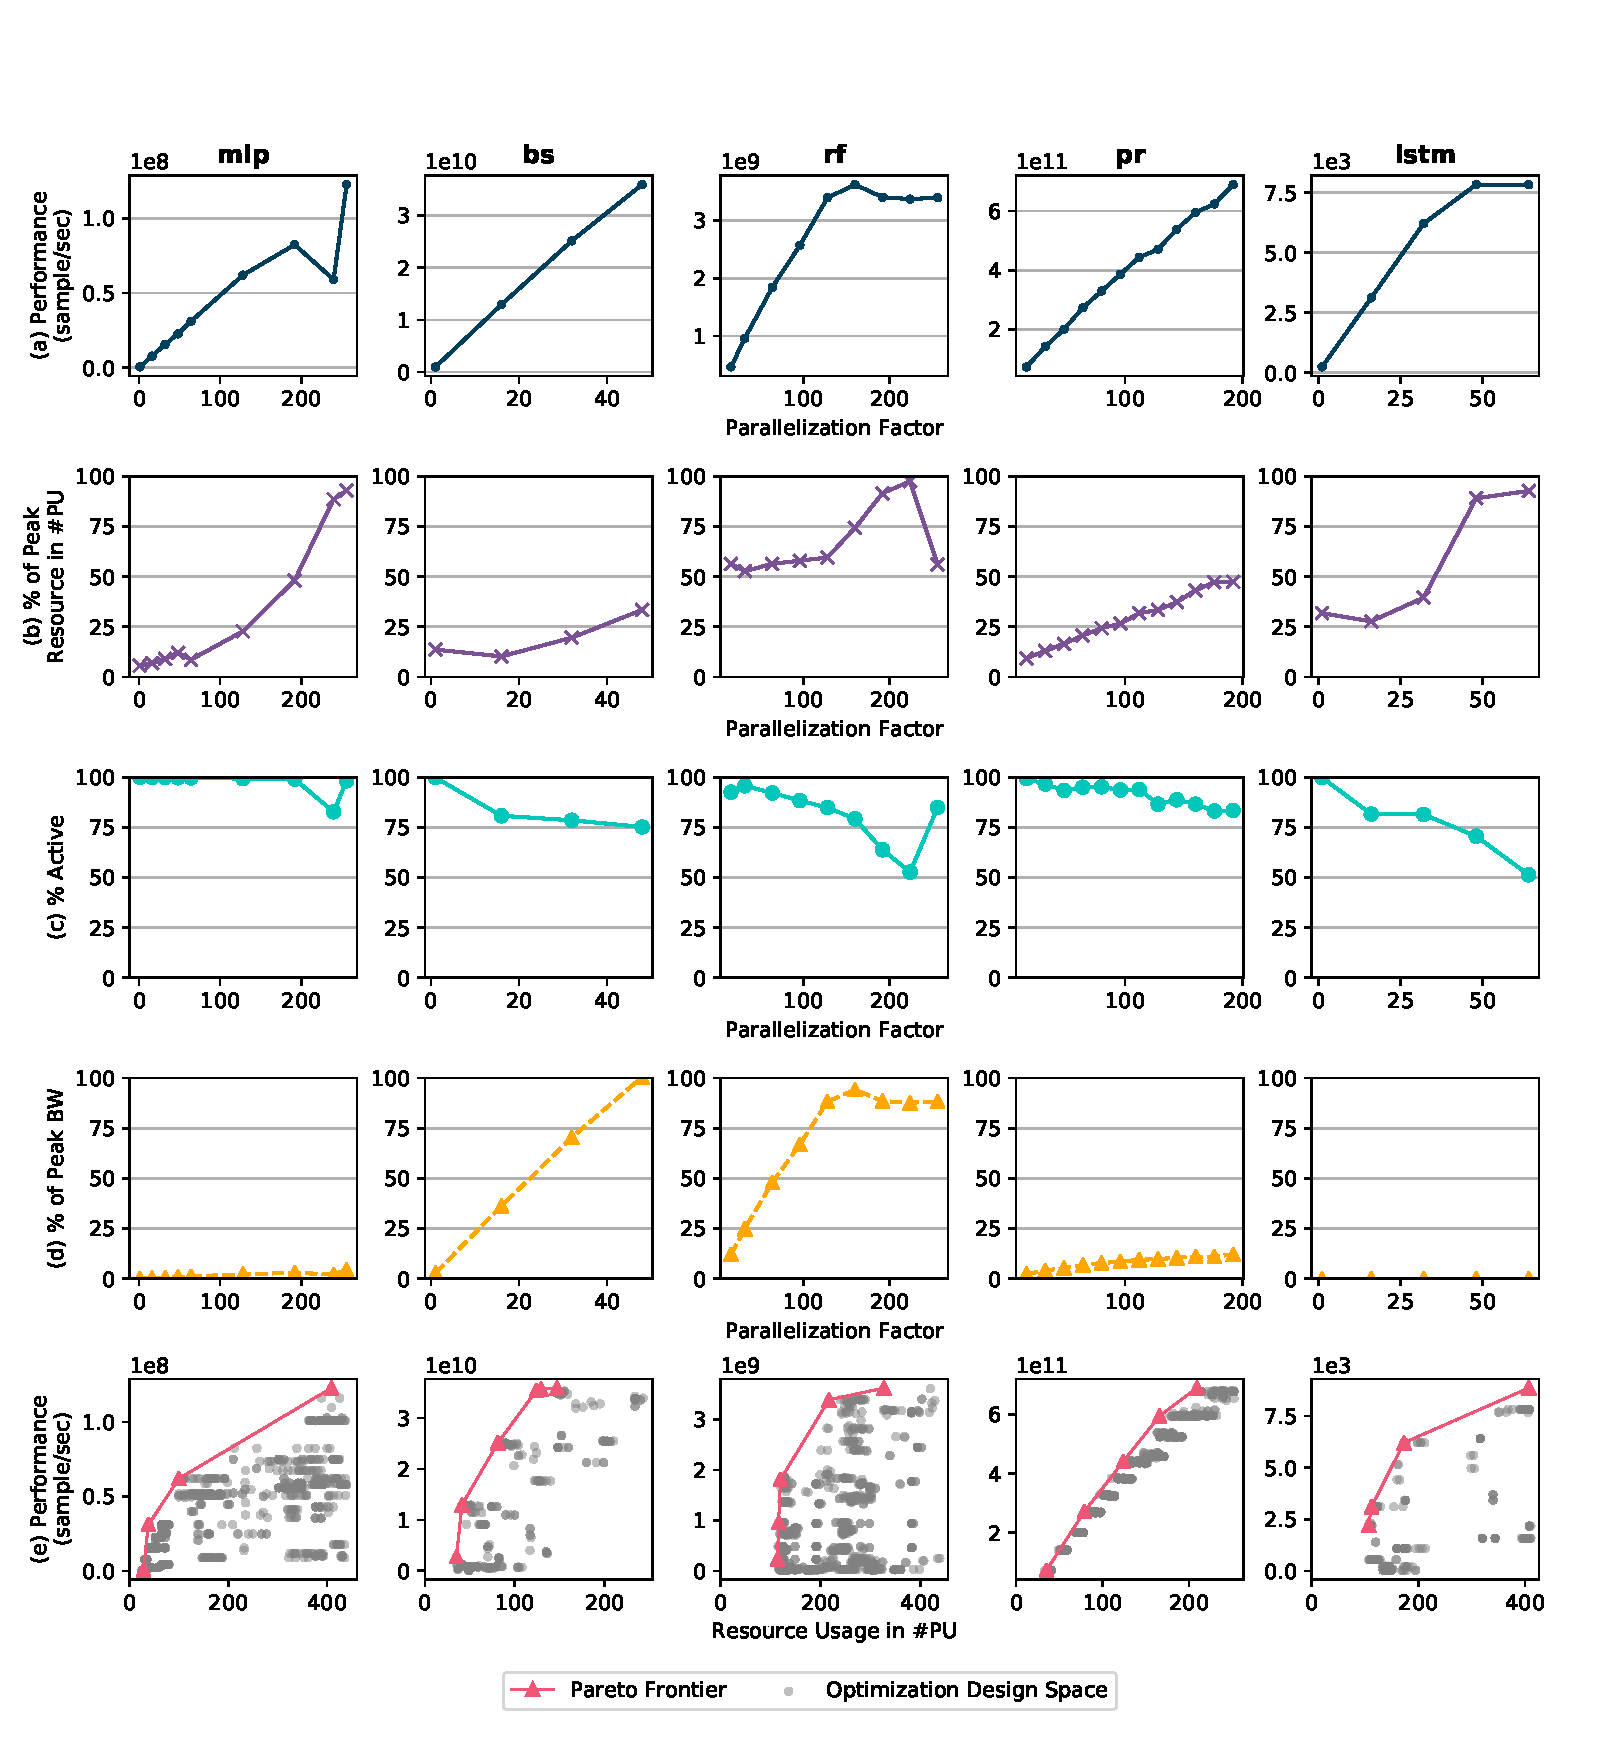
\includegraphics[width=1\textwidth]{/Users/yaqiz/pldi20/paper/figures/par_thesis.pdf}
\caption[Scalability evaluation]{
  Scalability evaluation. 
  Benchmarks include multi-layer perceptron (mlp), BlackScholes (bs), random forests (rf), page rank
  (pr), and long short-term memory recurrent neural network~\cite{hochreiter1997long}.
  The first four charts show the scaling of
  (a) throughput, 
  (b) resource usage, 
  (c) runtime activation rate of PUs on the critical path of the compute pipeline, 
  and (d) achieved HBM bandwidth, as the program gets parallelized.
  (e) shows the combined design space of compiler optimizations and parallelization factors on a
  throughput-resource curve. 
  The Pareto frontier presents the throughput improvement with an increasing resource by drawing the y-axis in (a) as a function of the y-axis in (b).
}
\label{fig:par}
\end{figure*}

\subsection{Scalability Evaluation}
\Cref{fig:par} shows how performance and on-chip resources vary as the application gets parallelized in
(a-d). 
For each parallelization factor, we evaluate a combination of various compiler flags, presenting the
best configurations in (a-d).
Starting with a non-parallelized and fully pipelined design, 
we incrementally parallelize the critical stages of the pipeline with the lowest throughput.
For \textbf{mlp}, for example, this corresponds to the dense layer with the most operations.
For DRAM-bound applications, like \textbf{rf}, we increase the number of parallel DRAM streams.
\Cref{fig:par} (a) shows an almost perfect performance scaling for most compute-bound apps, including
\textbf{mlp}, \textbf{bs}, and \textbf{lstm}.
The DRAM-bound applications, i.e. \textbf{rf} and \textbf{pr}, achieve a perfect scaling until
saturating in DRAM bandwidth, as shown in (c).

As we discussed in the MLP case study in \Cref{fig:mlp} and shown in (b), the resource does not
monotonically increase with parallelization factor due to optimizations discussed in \Cref{sec:opt},
which explains the dip in the \textbf{mlp} curve in (a). 
With further investigation, we found the best set of compiler flags that gives the perfect scaling 
did not fit in resource at parallelization factor of 240; hence, a flag combination using less
resource with less performance is presented. 
A design with the optimum flags consumes less resource at a higher parallelization factor at 256, 
as a power of two factor enables more optimizations, which continues the scaling.

The resource in (b) increases slowly with a small parallelization factor. This is because initially,
as the pipeline is highly imbalanced, \name only needs to parallelize a small portion of the
entire pipeline to improve overall throughput. As the pipeline gets balanced, \name must parallelize
all stages in the pipeline to further enhance throughput. Larger parallelization factor also comes
with the expensive crossbar connection from memory partitioning discussed in~\Cref{sec:memsplit}.

\Cref{fig:par} (c) shows the activation rate of the critical pipeline stages at runtime.
A close to 100\% activation rate at close to 100\% resources (400 PUs) suggests that 
\name introduces minimum synchronization overhead and is truly scalable.
The decreasing in the activation rate in \textbf{lstm} is due to increasing initiation interval
(II)~\cite{II} with large parallelization.
The recurrent neural network contains an inherent loop-carried dependency (LCD) in the algorithm. 
As we parallelize a stage with a reduction within the cycle of LCD, the latency of the reduction tree
also increases, resulting in a larger II that slows down the pipeline runtime.

\Cref{fig:par} (e) shows the full design space of performance-resource trade-off with
different parallelization factors and compiler optimizations.
We can see that compiler optimizations play an important role in improving performance or
reducing resource that pushes the Pareto leftwards and upwards.

\subsection{Comparison with a GPU}

\Cref{tab:gpu-comparison} shows the throughput and latency comparison with a Tesla V100 GPU.
\Cref{fig:speedup} presents the speedup with Plasticine.
In additional to raw measurements from simulation, we also present an area-normalized throughput
taking into account of the technology difference between Plasticine and V100 
for SqueezeNet 1.0~\cite{squeezenet} and LSTM~\cite{lstm}; 
these applications are compute-bound and hence their throughputs are proportional to available 
on-chip resources.

\begin{figure}
\begin{table}[H]
  \centering
    \footnotesize
    \begin{tabular}{lcccccc}
    \toprule
      \multirow{2}{*}{\textbf{Benchmark}} &
      \multirow{2}{*}{\makecell[c]{\bf Throughout\\\bf Unit}} &
      \multirow{2}{*}{\makecell[c]{\bf GPU\\\bf Compiler}} & \multicolumn{2}{c}{\textbf{Latency} (ms)} &
      \multicolumn{2}{c}{\textbf{Throughput} (Unit/s)} \\
                                & & & \name & GPU & \name & GPU     \\
      \midrule
        SqueezeNet (batch-1) & {\em kFrames}   & TF+cuDNN & 49.13  & 70.10  & 0.12 (1.1) & 0.4   \\ \addlinespace
        LSTM (batch-32)      & {\em kSamples}  & TF+cuDNN & 3.61   & 6.81   & 8.8 (79.2) & 4.7   \\ \addlinespace
        PageRank             & {\em MEdges}    & Gunrock & 128.27 & 829.39 & 49         & 7.5   \\ \addlinespace
        BlackScholes         & {\em GOptions}  & CUDA & 0.09   & 0.10   & 88.88      & 80.02 \\ \addlinespace
        Random Forest        & {\em MSamples}  & CUDA & 0.10   & 0.32   & 1.04       & 0.32  \\ \addlinespace
        Merge Sort           & {\em GElements} & CUDA & 0.63   & 2.14   & 6.65       & 1.96  \\
      \bottomrule
    \end{tabular}
  \caption[Performance comparison of Plasticine with a Tesla V100 GPU]{
Performance comparison of Plasticine with a Tesla V100 GPU (Normalized throughput to transistor count in parentheses).
}
  \label{tab:gpu-comparison}
\end{table}
\begin{figure}[H]
\centering
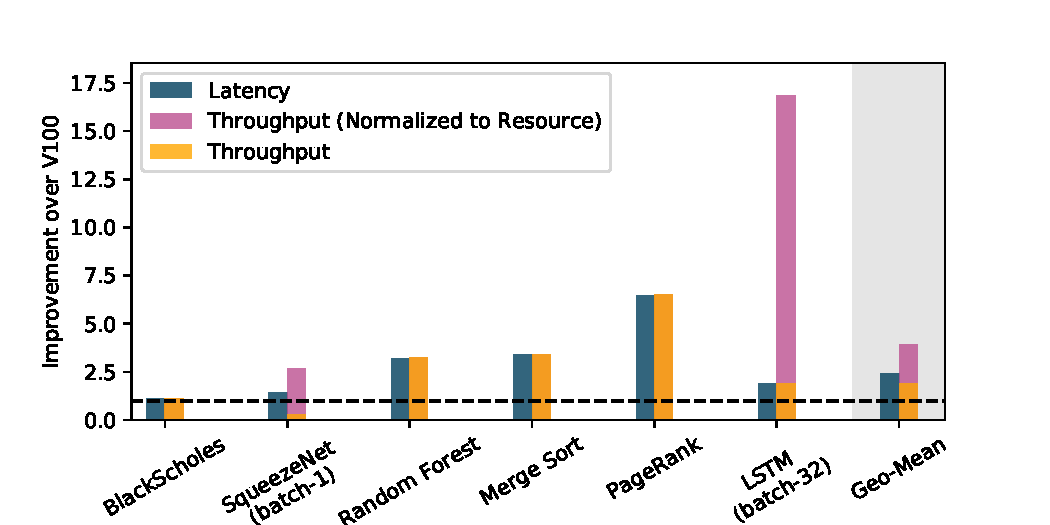
\includegraphics[width=1\textwidth]{figs/slide_gpu.pdf}
\caption[Performance comparison with a Tesla V100 GPU]{
  Plasticine's latency and throughout improvement over V100 GPU.
  The evaluated Plasticine architecture has area footprint of 352$mm^2$ at 28nm.
  V100 GPU has area footprint of 815$mm^2$ at 12nm.
  Both platforms have the same off-chip bandwidth at 1TB/s with HBM technology.
  Yellow and blue bars show the raw measured speedup in throughput and latency, respectively.
  To account for the resource discrepancy, the pink bar shows the normalized throughput
  for compute-bound application--SqueezeNet and LSTM, which scales performance with additionally
  on-chip resources.
}
\label{fig:speedup}
\end{figure}
\end{figure}

\paragraph{Neural Networks} 
After normalized in resource, Plasticine shows a 2.75x and 16.85x speedup in throughput for the
compute-bound applications--SqueezeNet and LSTM.
These applications benefit from the flexible degrees of parallelism \name{} exploits. 
In addition to streaming pipelining across network layers, \name can also parallelize on the
input and output channels/dimensions of a single convolution/dense layer in SqueezeNet/LSTM.
In contrast, GPU needs to accumulate a large batch size to fully utilize the parallel threads.
SqueezeNet also has a highly imbalanced pipeline, with 2x more computation in certain layers than
the others.
Exploiting pipeline parallelism allows Plasticine to distribute the most resources to the program
phase with the most operations.
GPU executes these layers in time and parallelizes them equally; 
layers with fewer operations are likely to underutilize the chip.

\paragraph{BlackScholes} 
Both Plasticine and V100 can saturate HBM2 bandwidth for BlackScholes.

\paragraph{PageRank} 
PageRank implemented in \name achieves a 6.5x latency speedup and throughput improvement comparing
to Gunrock \cite{gunrock} on the denaulay\_n20 \cite{delaunayn20} dataset. 
Due to the SIMT restriction in GPU, Gunrock only explore edge frontier parallelism, 
which underutilizes the hardware when the graph is sparse.
In contrast, \name{} parallelizes both the edge and node processing across multiple DRAM streams.
\name can exploit arbitrary levels of hierarchical parallelism on non-perfectly nested loops,
resulting in a perfect scaling of PageRank shown in~\Cref{fig:par} (a).

\paragraph{RandomForest} We created a synthesized tree model that contains 8 estimator trees and 128 splits per estimator. 
Implementation with \name{} on Plasticine shows 3.2x speedup comparing to the implementation in CUDA on V100. 
Similarly to BlackScholes, RandomForest contains a massive basic block with multiple tree
structures in the dataflow graph corresponding to the estimators.
GPU executes this basic block in time. 
As a result, the irregular memory access from the graph structure causes bad memory performance in V100.
In contrast, \name{} maps the entire dataflow graph spatially across PUs, vectorizing across a batch of 16 samples.
The entire basic block is streaming pipelined at full throughout without any memory access.

\paragraph{MergeSort} 
The merge tree implementation on Plasticine uses a multi-way merging tree to merge the sorted
partitions stored in the off-chip memory iteratively.
This implementation saturates off-chip bandwidth by parallelizing on multiple DRAM streams within
each iteration.
We compared merge sort and radix sort on GPU and took the radix sort with a faster runtime.
Overall, sorting on Plasticine implemented with \name provides 3.4x latency speedup and throughput
improvement against the GPU.

